\documentclass[12pt,compress,aspectratio=169]{beamer}

\usetheme{metropolis}
\setbeamersize{text margin left=.5cm,text margin right=.5cm}

\usefonttheme{professionalfonts}
\usepackage{amsmath}%,bm}
\usepackage{siunitx}
%\usepackage{graphicx}
\usepackage{tikz}
\usepackage{mathpazo}
\usepackage{xcolor,colortbl}
%\usepackage{hyperref}
%\usepackage{cancel}

\usetikzlibrary{decorations.pathmorphing,patterns}

\setsansfont{Roboto Light}
\setmonofont{Ubuntu Mono}
\setlength{\parskip}{0pt}
\setlength{\itemsep}{0pt}
\renewcommand{\baselinestretch}{1}

\sisetup{
  detect-all,
  %number-math-sf=\textsf,
  %number-math-rm=\mathnormal,
  per-mode=symbol
}

\title{Topic 5a: Gravity}
\subtitle{Advanced Placement Physics 1}
\author{Dr.\ Timothy Leung}
\institute{Olympiads School\\Toronto, Ontario, Canada}
\date{July 13, 2020}

\newcommand{\pic}[2]{\includegraphics[width=#1\textwidth]{#2}}
\newcommand{\mb}[1]{\ensuremath\mathbf{#1}}
\newcommand{\eq}[2]{\vspace{#1}{\Large\begin{displaymath}#2\end{displaymath}}}



\begin{document}

\begin{frame}
  \maketitle
\end{frame}


%\begin{frame}{Files to Download}
%  If you have not done so already, please download the following files.
%  \begin{itemize}
%  \item\texttt{PhysAP-08-Gravity-print.pdf}---The presentation slides for this
%    topic.
%  \item\texttt{PhysAP-08-Homework.pdf}---Homework questions for this topic.
%  \end{itemize}
%\end{frame}

\begin{frame}{Disclaimer}
  The section on circular motion and gravity only accounts for a small portion
  of the marks for Physics 1, but we spend more time on circular motion because
  it is important to our next topic. However, discussion on gravity will be
  limited. Some of the slides are repeats from Grade 12.
\end{frame}


\section{Gravitational Force}


\begin{frame}{Law of Universal Gravitation}
  \begin{center}
    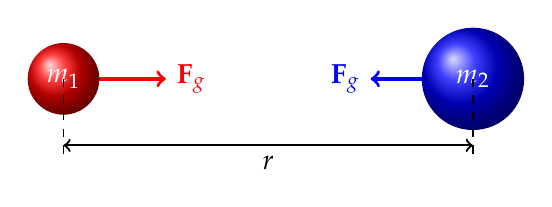
\begin{tikzpicture}[scale=.65]
      \draw[->,very thick,red](0,0)--(2,0) node[pos=1,right]{$\mb{F}_g$};
      \draw[->,very thick,blue](8,0)--(6,0) node[pos=1,left]{$\mb{F}_g$};
      \tikzstyle{balloon1}=[ball color=red];
      \tikzstyle{balloon2}=[ball color=blue];
      \shade[balloon1] (0,0) circle(.7) node[white]{$m_1$};
      \shade[balloon2] (8,0) circle(1) node[white]{$m_2$};
      \draw[dashed] (0,0)--(0,-1.5);
      \draw[dashed] (8,0)--(8,-1.5);
      \draw[<->,thick](0,-1.3)--(8,-1.3) node[midway,below]{$r$};
    \end{tikzpicture}
  \end{center}

  In classical mechanics, \textbf{gravity} is a mutually attractive force
  between massive objects, with a magnitude $F_g$ determined by the law of
  universal gravitation:

  \eq{-.2in}{
    \boxed{
      F_g=G\frac{m_1m_2}{r^2}
    }
  }

  where $G=\SI{6.674e-11}{\newton\metre\squared\per\kilo\gram\squared}$ is the \textbf{universal gravitation
    constant}, and $r$ is the distance between the centers of the masses.
  $m_1$ and $m_2$ are \emph{point masses} that do not occupy any space
\end{frame}



%\begin{frame}{Law of Universal Gravitation}
%  \begin{center}
%    \begin{tikzpicture}[scale=.5]
%      \draw[->,very thick,red](0,0)--(2,0) node[pos=1,right]{$\mb{F}_{21}$};
%      \draw[->,very thick,blue](8,0)--(6,0) node[pos=1,left]{$\mb{F}_{12}$};
%      \tikzstyle{balloon1}=[ball color=red];
%      \tikzstyle{balloon2}=[ball color=blue];
%      \shade[balloon1] (0,0) circle(.7) node[white]{$m_1$};
%      \shade[balloon2] (8,0) circle(1) node[white]{$m_2$};
%      \draw[dashed] (0,0)--(0,-1.5);
%      \draw[dashed] (8,0)--(8,-1.5);
%      \draw[->,thick](0,-1.3)--(8,-1.3) node[midway,below]{$\mb{r}_{12}$};
%    \end{tikzpicture}
%  \end{center}
%  \begin{itemize}
%  \item If $m_1$ exerts a gravitational force $\mb{F}_{12}$ on
%    $m_2$, then $m_2$ likewise also exerts a force of $\mb{F}_{21}=-\mb{F}_{12}$
%    on $m_1$. The two forces are equal in magnitude and opposite in direction
%    (third law of motion).
%  \item The (more familiar) scalar form is often used as well:
%
%    \eq{-.2in}{
%      \boxed{F_g=G\frac{m_1m_2}{r^2}}
%    }
%  \end{itemize}
%\end{frame}



\begin{frame}{More Than One Mass}
  \begin{columns}
    \column{.4\textwidth}
    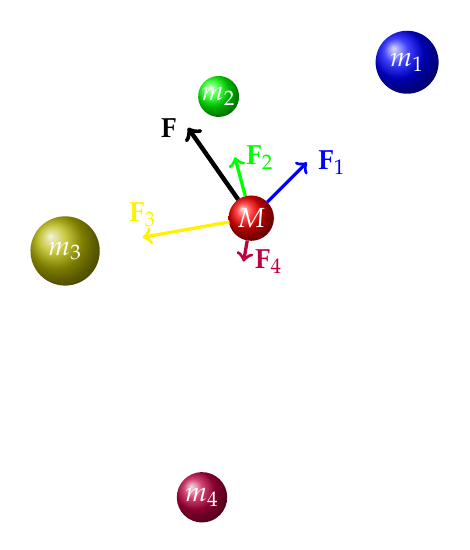
\begin{tikzpicture}[scale=.4]
      \tikzstyle{balloon1}=[ball color=red];
      \tikzstyle{balloon2}=[ball color=blue];
      \tikzstyle{balloon3}=[ball color=green];
      \tikzstyle{balloon4}=[ball color=yellow!70!black];
      \tikzstyle{balloon5}=[ball color=purple];
      \shade[balloon1] (0,0) circle(.72) node[white]{$M$};
      \begin{scope}[rotate=45]
        \draw[->,very thick,blue](.72,0)--(2.5,0) node[pos=1,right]{$\mb{F}_1$};
        \shade[balloon2] (7,0) circle(1) node[white]{$m_1$};
      \end{scope}
      \uncover<2->{
        \begin{scope}[rotate=105]
          \draw[->,very thick,green](.72,0)--(2,0)
          node[pos=1,right]{$\mb{F}_2$};
          \shade[balloon3] (4,0) circle(.65) node[white]{$m_2$};
        \end{scope}
      }
      \uncover<3->{
        \begin{scope}[rotate=190]
          \draw[->,very thick,yellow](.7,0)--(3.5,0)
          node[pos=1,above]{$\mb{F}_3$};
          \shade[balloon4] (6,0) circle(1.1) node[white]{$m_3$};
        \end{scope}
      }
      \uncover<4->{
        \begin{scope}[rotate=260]
          \draw[->,very thick,purple](.72,0)--(1.4,0)
          node[pos=1,right]{$\mb{F}_4$};
          \shade[balloon5] (9,0) circle(.8) node[white]{$m_4$};
        \end{scope}
      }
      \uncover<5>{
        \begin{scope}[rotate=125]
          \draw[->,ultra thick](.72,0)--(3.5,0) node[pos=1,left]{$\mb{F}$};
        \end{scope}
      }
    \end{tikzpicture}

    \column{.6\textwidth}
    For a mass $M$ that is subjected to the influence of multiple discrete point
    masses $m_i$, the total gravitational force that $M$ experiences
    is the vector sum of all the forces $\mb{F}_i$:
    
    \eq{-.25in}{
      \boxed{\mb{F}
        =\sum_i\mb{F}_i
        =GM\left(\sum_{i=1}^N\frac{m_i}{r_i^2}\hat{\mb{r}_i}\right)
      }
    }
  \end{columns}
\end{frame}



%\begin{frame}{Continuous Distribution of Mass}
%  At the limit $N\rightarrow\infty$, the summation becomes an integral, and can
%  now be used to describe the gravitational force from objects with
%  \emph{spatial extend} i.e.\ masses that take up space (e.g.\ a continuous
%  distribution of mass):
%
%  \eq{-.2in}{
%    \boxed{\mb{F}
%      =\int d\mb{F}
%      =GM\int\frac{dm}{r^2}\hat{\mb{r}}
%    }
%  }
%
%  Objects that are symmetrically spherical (e.g.\ planets are stars in our
%  solar system) can be treated as point masses, and integration can be avoided.
%  However, this is not necessarily the case for some celestial objects.
%\end{frame}



\section{Gravitational Field}

\begin{frame}{Gravitational Field}
  We generally describe the gravitational force (weight) as:
  
  \eq{-.2in}{
    \boxed{\mb{w}=\mb{F}_g=m\mb{g}}
  }

  To find $\mb{g}$, we group the variables in the law of universal gravitation:
    
  \eq{-.2in}{
    \mb{F}_g
    =\underbrace{\left[-\frac{Gm_1}{|\mb{r}|^2}\hat{\mb{r}}\right]}_{=\mb{g}}m
    =m\mb{g}
  }

  The vector field function $\mb{g}$ is known as the
  \textbf{acceleration due to gravity} in kinematics, and
  \textbf{gravitational field} in field theory.
\end{frame}



\begin{frame}{Gravitational Field}
  On/near the surface of Earth, we can use Earth's mass and radius

  \vspace{-.4in}{\Large
    \begin{align*}
      m_1&=\SI{5.972e24}{\kilo\gram}\\
      r&=\SI{6.371e6}{\metre}
    \end{align*}
  }
  
  \vspace{-.2in}to compute the commonly known value of

  \vspace{-.4in}{\Large
    \begin{align*}
      g &\approx\SI{9.81}{\metre\per\second^2}\\
      g &\approx\SI{9.81}{\newton\per\kilo\gram}
    \end{align*}
  }
\end{frame}



\begin{frame}{Gravitational Field}
  The \textbf{gravitational field} $\mb{g}$ generated by point mass $m$
  shows how it influences the gravitational forces on other masses:

  \eq{-.2in}{
    \boxed{g(m,\mb{r})=-\frac{Gm}{|\mb{r}|^2}\hat{\mb{r}}}
  }
  \begin{center}
    \begin{tabular}{l|c|c}
      \rowcolor{pink}
      \textbf{Quantity} & \textbf{Symbol} & \textbf{SI Unit} \\ \hline
      Gravitational field       & $\mb{g}$ & \si{\newton\per\kilo\gram}\\
      Universal gravitational constant
      & $G$ & \si{\newton\metre^2/\kilo\gram^2} \\
      Source mass               & $m$ & \si{\kilo\gram} \\
      Distance from source mass & $|\mb{r}|$ & \si{\metre}\\
      Outward radial unit vector from source & $\hat{\mb{r}}$ & N/A
    \end{tabular}
  \end{center}
  The \emph{direction} of the gravitational field is toward $m$ (that's why the
  negative sign)
\end{frame}



\begin{frame}{More Than One Mass}
  When there are multiple point masses present, the total gravitational field
  at any position $\mb{r}$ is the vector sum of all the fields $\mb{g}_i$:
    
  \eq{-.2in}{
    \boxed{\mb{g}
      =\sum_i\mb{g}_i
      =G\left(\sum_i\frac{m_i}{r_i^2}\hat{\mb{r}_i}\right)
    }
  }
\end{frame}




\begin{frame}{Relating Gravitational Field \& Gravitational Force}
  $\mb{g}$ acts on any mass $m$ that enters the field. Then, $m$ experiences a
  gravitational force $\mb{F}_g$, regardless of how $\mb{g}$ is created:

  \eq{-.2in}{
    \boxed{\mb{F}_g=m\mb{g}}
  }
  \begin{center}
    \begin{tabular}{l|c|c}
      \rowcolor{pink}
      \textbf{Quantity} & \textbf{Symbol} & \textbf{SI Unit} \\ \hline
      Gravitational force on a mass & $\mb{F}_g$ & \si{\newton} \\
      Mass inside the gravitational field & $m$ & \si{\kilo\gram}\\
      Gravitational field & $\mb{g}$   & \si{\newton\per\kilogram}
    \end{tabular}
  \end{center}
  Note: A point mass is not affected by the gravitational field that itself
  generates.
\end{frame}



\begin{frame}{Inside A Spherical Shell?}
  \begin{columns}
    \column{.3\textwidth}

    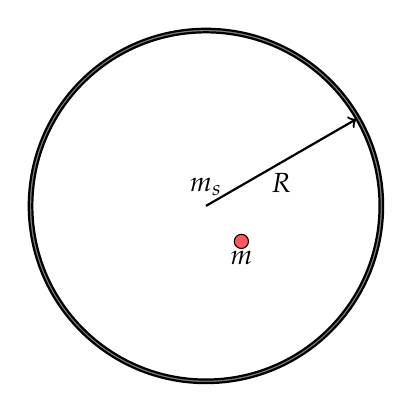
\begin{tikzpicture}[scale=.45]
      \draw[thick,fill=gray](0,0) circle(5) node[above]{$m_1$};
      \draw[thick,fill=white](0,0) circle(4.9) node[above]{$m_s$};
      \draw[thick,->,rotate=30](0,0)--(4.9,0) node[midway,below]{$R$};
      \draw[fill=red!65](1,-1) circle(.2) node[below]{$m$};
    \end{tikzpicture}

    \column{.7\textwidth}
    It can be shown mathematically theatthe gravitational field \emph{inside} a
    spherical hollow shell is zero:
      
    \eq{-.2in}{
      \boxed{
        \mb{g}=
        \begin{cases}
          \mb{0} & \text{if}\;\;r<R\\
          -Gm_s/r^2\hat{\mb{r}} & \text{otherwise}
        \end{cases}
      }
    }
    
    A mass $m$ \emph{inside} the shell experiences no gravitational force from
    the shell.
  \end{columns}
\end{frame}


%\begin{frame}{What If You Are Inside Another Mass?}{Uniform Mass of Radius $R$}
%  \begin{columns}
%    \column{.35\textwidth}
%
%    \begin{tikzpicture}[scale=.45]
%      \draw[thick,fill=gray!50](0,0) circle(5);
%      \clip(-.2,-6) rectangle (.2,6);
%      \draw[very thick](.2,5)--(.2,-5);
%      \draw[very thick](-.2,5)--(-.2,-5);
%      \draw[fill=red!65](0,1) circle(.15) node[right]{$m_2$};
%    \end{tikzpicture}
%
%    \column{.65\textwidth}
%    Suppose you could drill a hole through the Earth and then jump into it. How
%    long would it take you to emerge on the other side of the Earth?
%
%    \vspace{.2in}To calculate this, we need to know how the gravitational force
%    changes as you fall through Earth.
%  \end{columns}
%\end{frame}
%
%
%
%\begin{frame}{Falling Toward the Center of Earth}
%  \begin{columns}
%    \column{.3\textwidth}
%    \pic{1}{eartholeg.png}
%
%    \column{.7\textwidth}
%    As you fall through Earth, we can separate the part of Earth that is
%    ``above'' you, and the part that is ``below'' you
%    \begin{itemize}
%    \item The part that is ``above'' you is like the spherical shell, and does
%      not contribute to the gravitational field, and therefore does not exert
%      any force
%    \item The part that is ``below'' you gets smaller as you fall toward the
%      center
%    \end{itemize}
%  \end{columns}
%\end{frame}
%
%
%
%\begin{frame}{Falling Toward the Center of Earth}
%  Assuming that Earth's density is uniform, and neglecting air resistance and
%  other factors, the value of $g$ as the person falls through Earth ($r<R$) is
%  given by finding how much mass is still ``below'' the person, $M(r)$:
%
%  \eq{-.1in}{
%    g(r)=\frac{GM(r)}{r^2}\quad M(r)=\frac{4}{3}\rho\pi r^3\quad
%    \rho=\frac{3M_\oplus}{4\pi r_\oplus^3}
%  }
%
%  where $M_\oplus$ is the mass of Earth, $r_\oplus$ is the radius of Earth,
%  $\rho$ is the (constant) density, and $r$ is the distance from Earth's
%  center. Then $M(r)$ is the amount of mass ``below'' the person as he/she
%  falls toward the center.
%\end{frame}
%
%
%
%\begin{frame}{Falling Toward the Center of Earth}
%  \vspace{.2in}
%  \begin{columns}
%    \column{.25\textwidth}
%    \pic{1.2}{eartholeg.png}
%
%    \column{.75\textwidth}
%    The gravitational field strength inside this hypothetical Earth is a
%    linear function of distance $r$ from the center:
%
%    \eq{-.2in}{
%      g(r)=\frac{GM_\oplus r}{r_\oplus^3}=\left[\frac{g_0}{r_\oplus}\right]r
%    }
%    
%    where $g_0=\SI{9.81}{\newton\per\kilogram}$ is the field strength at the
%    surface. At the center ($r=0$), $g=0$. The gravitational force is:
%    
%    \eq{-.2in}{
%      F_g(r)=-\underbrace{\left[\frac{mg_0}{r_\oplus}\right]}_{k} r
%    }
%  \end{columns}
%\end{frame}
%
%
%
%\begin{frame}{Falling Toward the Center of Earth}
%  \begin{columns}
%    \column{.25\textwidth}
%    \pic{1}{eartholsat.png}
%
%    \column{.75\textwidth}
%    The gravitational force has the same form as Hooke's law: it is
%    proportional to displacement from the center, but in the opposite
%    direction:
%
%    \eq{-.2in}{
%      F_g(r)=-kr
%    }
%    
%    \vspace{-.15in}The motion is a simple harmonic motion. The traveller will
%    oscillate through Earth with a period of:
%
%    \eq{-.2in}{
%      T=2\pi\sqrt{\frac{m}{k}}=2\pi\sqrt{\frac{r_\oplus}{g_0}}
%    }
%
%    For Earth, $T=\SI{5068}{\second}$. The traveller would pop up on the
%    opposite side every \SI{42}{min}.
%  \end{columns}
%\end{frame}
%
%
%
%
%\begin{frame}{Falling Toward the Center of Earth}
%  \begin{columns}
%    \column{.25\textwidth}
%    \pic{1}{eartholsat.png}
%
%    \column{.75\textwidth}
%    Since simple harmonic motion is a projection of a uniform circular motion,
%    if a satellite is in a circular orbit just above the surface, and passes
%    overhead just above the traveller as he/she popped up out of the hole. The
%    period of such an orbit would be the same as oscillating traveller.
%  \end{columns}
%\end{frame}



\begin{frame}{Gravitational Field Lines}
  \begin{center}
    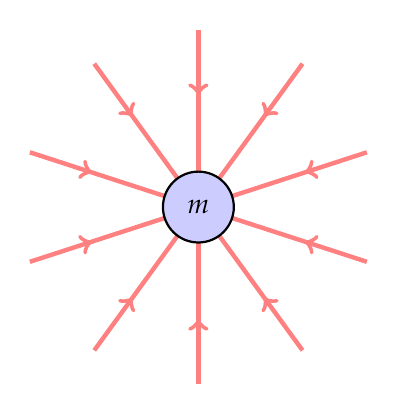
\begin{tikzpicture}[scale=1.5]
      \foreach \x in {0,...,9}\draw[red!50,ultra thick,rotate=36*\x](0,0)--(0,1);
      \foreach \x in {0,...,9}
      \draw[red!50,<-,ultra thick,rotate around={36*\x:(0,0)}](0,.95)--(0,1.5);
      \draw[fill=blue!20,thick](0,0) circle(.3) node{$m$};
    \end{tikzpicture}
  \end{center}
  \begin{itemize}
  \item The direction of $\mb{g}$ is toward the center of the object that
    created it
  \item Field lines do not tell the intensity (i.e.\ magnitude) of $\mb{g}$,
    only the direction
  \end{itemize}
\end{frame}



\begin{frame}{Gravitational Field Lines}
  When there are multiple masses, the total gravitational field (dotted line)
  is the vector sum of all the individual fields.
  \begin{center}
    \pic{.4}{grav-fields.png}
  \end{center}
  The solid lines are called \textbf{equipotential lines}, where the potential
  energy is constant. Equipotential lines are perpendicular to
  gravitational field lines.
\end{frame}



\section{Gravitational Potential Energy}

\begin{frame}{Gravitational Potential Energy}
  The expression for \textbf{gravitational potential energy} can be obtained
  from the law of universal gravitation using some basic calculus:

  \eq{-.2in}{
    \boxed{U_g=-G\frac{m_1m_2}{r}}
  }
  \begin{itemize}
  \item $U_g$ is the work required to move two objects from $r$ to $\infty$
  \item $U_g=0$ at $r=\infty$ and \emph{decrease} as $r$ decreases
  \item The fundamental theorem of calculus shows that the direction of
    gravitational force $\mb{F}_g$ always points from high to low potential
    energy,
    \begin{itemize}
    \item A free-falling object is always decreasing in $U_g$, while
    \item Objects traveling $\perp$ to $\mb{F}_g$ has constant $U_g$
    \end{itemize}
  \end{itemize}
\end{frame}



%\begin{frame}{Relating $U_g$, $\mb{F}_g$ and $\mb{g}$}
%  Knowing that $\mb{F}_g$ and $\mb{g}$ only differ by a constant (mass $m$), we
%  can also relate gravitational field to potential energy by the gradient
%  operator:
%
%  \eq{-.15in}{
%    \mb{g}%=\frac{\mb{F}_g}{m}=
%    =-\nabla V_g=-\frac{\partial V_g}{\partial r}\hat{\mb{r}}
%    \quad\text{where}\quad
%    V_g=\frac{U_g}{m}
%  }
%
%  We already know that the direction of $\mb{g}$ is the same as $\mb{F}_g$,
%  i.e.
%  \begin{itemize}
%  \item The direction of $\mb{g}$ is the shortest path to decrease $U_g$ 
%  \item Objects traveling perpendicular to $\mb{g}$ has constant $U_g$
%  \item $V_g$ is called the \textbf{gravitational potential} but
%    it is rarely used
%  \end{itemize}
%\end{frame}



\section{Orbital Motion}
%\begin{frame}{Orbital Mechanics \& Kepler's Laws of Planetary Motion}
%  In Physics 12, you studied briefly at the orbits of satellites around Earth,
%  or the orbit of Earth and other planets around the Sun.
%  \begin{itemize}
%  \item Used your understanding of centripetal motion and gravity
%  \item Assumed a circular orbit
%  \end{itemize}
%  Let's review some of those ideas.
%\end{frame}

%\subsection{Orbital Velocity}

\begin{frame}{Newton's Thought Experiment}
  In \emph{Treatise of the System of the World}, the third book in
  \emph{Principia}, Newton presented this thought experiment:
  \begin{center}
    \pic{.8}{figure-5.png}
  \end{center}
  \begin{itemize}
  \item How fast does the cannonball have to travel before it goes around Earth
    without falling? (i.e.\ goes into orbit)
  \item How fast does the cannonball have to travel before it never comes back?
  \end{itemize}
\end{frame}



\begin{frame}{Relating Gravitational and Centripetal Force}
  Assuming a small mass $m$ in circular orbit around a much larger mass $M$.
  The required centripetal force is supplied by the gravitational force:
  
  \eq{-.2in}{
    F_g=F_c\quad\longrightarrow\quad \frac{GMm}{r^2}=\frac{mv^2}{r}
  }

  \vspace{-.1in}Solving for $v$, we obtain the \textbf{orbital velocity}
  $v_{\text{orb}}$ which does not depend on the mass of the small object in
  orbit:

  \eq{-.15in}{
    \boxed{v_{\text{orb}}=\sqrt{\frac{GM}{r}}}
  }

  \vspace{-.1in}This equation is only applicable for perfectly circular orbits.
  (The orbital velocity equation is not part of the equation sheet, but it may
  be very easy to derive.)
\end{frame}



\subsection{Escape Velocity}

\begin{frame}{Escape Velocity}
  An object can leave the surface of Earth at any speed. But when all the
  kinetic energy of that object is converted to gravitational potential energy,
  it will return back to the surface of the earth. There is, however, a
  \emph{minimum} velocity at which the object \emph{would not} fall back to
  Earth.
\end{frame}



\begin{frame}{Escape Velocity}
  The calculation for escape velocity is an exercise in conservation of energy,
  since gravity is a conservative force, i.e.:

  \eq{-.2in}{
    K + U_g = K' + U_g'
  }
  \begin{itemize}
  \item\vspace{-.1in}Initial gravitational potential energy at the surface is:

    \eq{-.15in}{
      U_g=-\frac{GMm}{r_i}
    }
  \item Final gravitational potential energy is at the other side of the
    universe ($r=\infty$), where $U_g'=0$. At this point, the object has
    \emph{escaped} the gravitational pull of the planet/star
  \item The minimum kinetic energy at $r=\infty$ is $K'=0$
%  \item The work against gravity converts kinetic energy into gravitational
%    potential energy.
%  \item If you start with \emph{more} kinetic energy than required to do all
%    the work, then the object has
%    planet.
  \end{itemize}
\end{frame}



\begin{frame}{Escape Velocity from Circular Orbits}
  Set $K$ to equal to $-U_g$:

  \eq{-.25in}{
    \frac12mv_i^2=\frac{GMm}{r_i}
  }

  We can then solve for the initial speed $v_i=v_{\text{esc}}$ (called the
  \textbf{escape velocity}):

  \eq{-.2in}{
    \boxed{v_{\text{esc}}=\sqrt{\frac{2GM}{r_i}}}
  }

  where $r_i$ is the initial distance from the center of the planet/star, and
  it does not have to be on the surface.
\end{frame}



%\begin{frame}{Example Problem}
%  \textbf{Example:} Determine the escape velocity and energy for a
%  \SI{1.60e4}{\kilo\gram} rocket leaving the surface of Earth.
%
%  \uncover<2>{
%    \vspace{.5in}Note: The equation for the escape speed is based on the object
%    have a \emph{constant} mass, which is \emph{not} the case for a rocket
%    going into space.
%  }
%\end{frame}



%\begin{frame}{What if I'm not escaping from the surface?}
%  Both objects have the same escape velocity:
%  \begin{center}
%    \begin{tikzpicture}[scale=1.3]
%      \draw[fill=blue!80](0,0) circle(0.2) node[midway,below]{\tiny $M$};
%      \draw[dotted,thick] (0,0) circle(1);
%      \fill[black!70](0,1) circle(.03);
%      \draw[->,thick](0,0)--(0,.98) node[midway,right]{\tiny $r$};
%      \fill[black!70](2,0) circle(.03);
%      \draw[->,dash dot](0,1) to[out=0,in=135](2,0);
%    \end{tikzpicture}
%    \hspace{.3in}
%    \begin{tikzpicture}[scale=1.3]
%      \draw[fill=blue!20] (0,0) circle(1) node[midway,below]{\tiny $M$};
%      \fill[black!70](0,1) circle(0.03);
%      \draw[->,thick](0,0)--(0,.98) node[midway,right]{\tiny $r$};
%      \fill[black!70](2,0) circle(0.03);
%        \draw[->,dash dot](0,1) to[out=0,in=135](2,0);      
%    \end{tikzpicture}
%  \end{center}
%  The difference is that the object in orbit (left) already has orbital speed
%  $v_\mathrm{orbit}$, so escaping from that orbit requires only an additional
%  speed of
%  
%  \eq{-.2in}{
%    \Delta v=v_\mathrm{esc}-v_\mathrm{orbit}=(\sqrt{2}-1)v_\mathrm{orbit}
%  }
%  \begin{itemize}
%  \item What if $v_\mathrm{orbit}<v<v_\mathrm{esc}$?
%  \item What if $v<v_\mathrm{orbit}$?
%  \end{itemize}
%\end{frame}



%\begin{frame}{Non-Circular Orbits}
%  \begin{center}
%    \pic{.6}{newton-cannon-orbital-types-Seeds.jpg}
%  \end{center}
%\end{frame}



\subsection{Orbital Energies}

\begin{frame}{Orbital Energies}
  We can obtain the \textbf{orbital kinetic energy} in a perfectly circular
  orbit by using the orbital speed in our expression of kinetic energy:

  \eq{-.2in}{
    K_{\text{orb}}=\frac12mv_{\text{orb}}^2=\frac12m
    \left(\sqrt{\frac{GM}{r}}\right)^2=\boxed{\frac{GMm}{2r}}
  }

  We already have an expression for gravitational potential energy:

  \eq{-.15in}{
    U_g=-\frac{GMm}{r}=-2K_\mathrm{orbit}
  }
\end{frame}



\begin{frame}{Orbital Energies}
  \vspace{-.1in}The \textbf{total orbital energy} is the sum of $K$ and $U_g$:

  \eq{-.15in}{
    E_T=K_{\text{orb}}+U_g=-\frac{GMm}{2r}=-K_{\text{orb}}
  }

  Note the relationship:

  \eq{-.2in}{
    K=-\frac12U_g=-E_T
  }

  You are unlikely to encounter this in an AP exam, but this relationship, when
  applied to \emph{electrostatic} force, was crucial in developing the first
  model for the hydrogen atom
\end{frame}



%\section{Orbital Mechanics}
%
%\begin{frame}{Orbital Mechanics}
%  \textbf{The following slides for orbital mechanics are only presented as a
%    reference. Understanding this material require you to first learn about
%    angular momentum, which is the next topic in the course.}
%\end{frame}
%
%
%
%\begin{frame}{Properties of Gravitational Force}
%  Two properties of gravity are crucial to understanding of orbital mechanics:
%  \begin{enumerate}
%  \item Gravity is a \emph{conservative force}, in that
%    \begin{itemize}
%    \item The total mechanical energy of objects under gravity is constant
%    \item Work done by gravity converts gravitational potential energy $U_g$
%      into kinetic energy $K$; work against gravity converts $K$ into $U_g$
%    \end{itemize}
%  \item Gravity is a \emph{central force}, in that
%    \begin{itemize}
%    \item Gravitational force $\mb{F}_g$ is always in the $-\hat{\mb{r}}$
%      direction, i.e.\ $\mb{F}\times\mb{r}=\mb{0}$
%    \item Therefore gravity doesn't generate any torque
%    \item And therefore angular momentum $\mb{L}$ is constant
%    \end{itemize}
%  \end{enumerate}
%  These two properties are true regardless of the shape of the orbit, and even
%  for objects that are not in orbit at all.
%\end{frame}
%
%
%\begin{frame}{Kepler's Laws of Planetary Motion}
%  Johannes Kepler (1571--1630) formulated the \textbf{laws of planetary motion}
%  between 1609 to 1619, by interpreting planetary motion data from his teacher,
%  Tycho Brahe. It is an improvement over the heliocentric theory of Nicolaus
%  Copernicus. Expressed in modern language:
%  \begin{enumerate}
%  \item\textbf{Law of ellipses:} The orbit of a planet is an ellipse with the
%    Sun at one of the two foci.
%  \item\textbf{Law of equal areas:} A line segment joining a planet and the Sun
%    sweeps out equal areas during equal intervals of time
%  \item \textbf{Law of periods:} The square of the orbital period of a planet
%    is proportional to the cube of the semi-major axis of its orbit.
%  \end{enumerate}
%  (For anyone who is interested, there is a handout with the proofs of Kepler's
%  laws using Newton's laws of motion.)
%\end{frame}
%
%
%
%\subsection{Second Law}
%
%\begin{frame}{Kepler's Second Law: Law of Equal Areas}
%  \begin{center}
%    \fbox{
%      \begin{minipage}{.97\textwidth}
%        \textbf{Law of Equal Areas: A line segment joining a planet and the Sun
%          sweeps out equal areas during equal intervals of time}
%      \end{minipage}
%    }
%
%    \pic{.4}{201532-132212364-3243-planet.png}
%  \end{center}
%  The second law of planetary motion is the easiest to proof, by applying the
%  conservation of angular momentum $\mb{L}=m(\mb{r}\times\mb{v})$ (gravity is a
%  central force).
%\end{frame}
%
%
%
%\begin{frame}{Kepler's Second Law: Law of Equal Areas}
%  \begin{center}
%    \fbox{
%      \begin{minipage}{.9\textwidth}
%        \textbf{A line segment joining a planet and the Sun sweeps out equal
%          areas during equal intervals of time}
%      \end{minipage}
%    }
%  \end{center}
%  \begin{columns}
%    \column{.3\textwidth}
%    \begin{tikzpicture}[scale=1.3]
%      \fill[gray!45](0,0)--(2,3)--(3,2.8)--cycle;
%      \node at (1.7,2) {$d\mb{A}$};
%      \draw[->,thick](0,0)--(2,3)
%      node[midway,left]{$\mb{r}$} node[pos=.95,right]{$\alpha$};
%      \draw[->,thick](2,3)--(3,2.8) node[midway,above]{$d\mb{r}$};
%      \draw[dashed](3,2.8)--(0,0);
%      \fill[black](0,0) circle(.07) node[right]{\tiny\text{Sun}};
%      \fill[black](2,3) circle(.035)node[above]{\tiny\text{Planet}};
%    \end{tikzpicture}
%    \column{.7\textwidth}
%    The infinitesimal area $d\mb{A}$ swept out by an object (such as a planet)
%    as it moves in orbit by an infinitesimal amount $d\mb{r}$ is given by:
%    
%    \eq{-.4in}{
%      dA=\frac{1}{2}rdr\sin\alpha
%      \;\rightarrow\;
%      d\mb{A}=\frac{1}{2}\mb{r}\times d\mb{r}
%    }
%
%    \vspace{-.15in}Its time derivative is called the \textbf{areal velocity}:
%      
%    \eq{-.15in}{
%      \frac{d\mb{A}}{dt}
%      =\frac{1}{2}\mb{r}\times\frac{d\mb{r}}{dt}
%      =\frac{1}{2}\mb{r}\times\mb{v}
%    }
%  \end{columns}
%\end{frame}
%
%
%
%\begin{frame}{Kepler's Second Law: Law of Equal Areas}
%%  We can express $\mb{r}\times\mb{v}$ in terms of angular momentum,
%%  $\mb{L}=m(\mb{r}\times\mb{v})$. But in motion under any central force (such
%%  as gravity), angular momentum is a constant, and therefore: 
%  The rate of change of the area ($dA/dt$) swept out by a planet (called the
%  \textbf{areal velocity}) is given by:
%
%  \eq{-.15in}{
%    \frac{dA}{dt}
%    =\frac{L}{2m}=\text{constant}
%  }
%
%  The rate a planet sweeps out the area in orbit is its angular momentum around
%  the sun divided by twice its mass.
%\end{frame}
%
%
%
%\subsection{First Law}
%
%\begin{frame}{Kepler's First Law: Law of Ellipses}
%  Proofing Kepler's first law requires some understanding the ellipse. If
%  the law is true, then orbital motion must agree with the equations of an
%  ellipse.
%  \begin{columns}
%    \column{.3\textwidth}
%    \begin{center}
%      \pic{1.25}{elliporb.png}
%    \end{center}
%
%    \column{.7\textwidth}
%    \begin{itemize}
%    \item $r' + r =2a$
%    \item The area of the ellipse is $A=\pi ab$
%    \item The relationship between $r$ and $\theta$ given by:
%
%      \eq{-.35in}{
%        r=\frac{a(1-e^2)}{1+e\cos\theta}
%        \quad\textnormal{\normalsize where}\quad
%        0\leq e < 1
%      }
%    \item when $e=0$ it's a circle: $a=b=r$
%    \item When $e=1$ it's no longer an ellipse
%    \end{itemize}
%  \end{columns}
%\end{frame}
%
%
%
%\begin{frame}{Kepler's First Law: Law of Ellipses}
%  \begin{columns}
%    \column{.6\textwidth}
%    Most planets in the solar system have very small eccentricity, so their
%    orbits are fairly close to being circular, but comets are much more
%    eccentric
%    \begin{center}
%      \pic{.65}{kep5.png}
%    \end{center}
%    
%    \column{.4\textwidth}
%    \begin{tabular}{l|l}
%      \rowcolor{pink}
%      \textbf{Object} & $e$ \\ \hline
%      Mercury	& \num{.206} \\
%      Venus	& \num{.0068} \\
%      Earth	& \num{.0167} \\
%      Mars	& \num{.0934} \\
%      Jupiter	& \num{.0485} \\
%      Saturn	& \num{.0556} \\
%      Uranus	& \num{.0472} \\
%      Neptune	& \num{.0086} \\
%      Pluto	& \num{.25} \\ \hline
%      Halley's Comet   & \num{.9671} \\
%      Comet Hale-Bopp  & \num{.9951} \\
%      Comet Ikeya-Seki & \num{.9999}
%    \end{tabular}
%  \end{columns}
%\end{frame}
%
%
%
%\begin{frame}{Kepler's First Law: Law of Ellipses}
%  As $m$ orbits around $M$, there are two velocity components:
%  \textbf{radial velocity} $\mb{v}_r$ and \textbf{angular velocity}
%  $\mb{v}_\theta$.
%  \begin{columns}
%    \column{.3\textwidth}
%    \begin{tikzpicture}[scale=.55]
%      \def\a{4} % semi-major axis
%      \def\b{3.25} % semi-minor axis
%      \def\angle{150} % angle
%      \draw (0,0) ellipse ({\a} and {\b});% Draw the ellipse
%      \draw ({sqrt(\a*\a-\b*\b)},-2.65)--({sqrt(\a*\a-\b*\b)},2.65);
%      \draw (-\a-.2,0)--(\a+.2,0);
%      \fill[black]({sqrt(\a*\a-\b*\b)},0) circle(.1)
%      node[below right]{\tiny $M$};
%      \begin{scope}[rotate around={\angle:({sqrt(\a*\a-\b*\b)},0)}]
%        \draw[->]({sqrt(\a*\a-\b*\b)},0)--(8.5,0)
%        node[pos=.45,below]{\tiny$\mb{r}$}
%        node[pos=1,left]{\tiny $\mb{v}_r$};
%        \draw[->](7.65,0)--(7.65,.85) node[below]{\tiny $\mb{v}_\theta$};
%        \fill (7.65,0) circle(.1) node[above]{\tiny $m$};
%      \end{scope}
%      \draw[->]({sqrt(\a*\a-\b*\b)+.5},0) arc(0:\angle:.5)
%      node[pos=.4,above]{\tiny$\theta$};
%%      \draw[<->]({sqrt(\a*\a-\b*\b)-.2},0)--({sqrt(\a*\a-\b*\b)-.2},-2.65)
%%      node[midway,left]{\tiny$r_0$};
%    \end{tikzpicture}
%    
%    \column{.7\textwidth}
%    \begin{itemize}
%    \item $\mb{v}_\theta$ means a centripetal acceleration toward $M$
%    \item Changes in $\mb{v}_r$ (i.e.\ accceleration in the radial direction)
%      also means a force along $\hat{\bm{r}}$
%    \item Both components of acceleration are due entirely to gravitational
%      force toward $M$
%    \item Applying second law of motion gives a complicated (at least for
%      students new to the concept) ordinary differential equation.
%    \end{itemize}
%  \end{columns}
%  \vspace{.1in}A full description for solving the differential equation is
%  presented in the accompanied handout for anyone interested.
%\end{frame}
%
%
%
%\begin{frame}{Kepler's First Law: Law of Ellipses}
%  The solution to the ODE is the expression for $r(\theta)$, with eccentricity
%  $e$ determined by a constant $B$ based on initial condition (how the planet
%  is formed):
%
%  \eq{-.2in}{
%    r%=\frac{1}{\frac{GMm^2}{L^2}(1+e\cos\theta)}
%    =\left[\frac{L^2}{GMm^2}\right]\frac{1}{1+e\cos\theta}
%    \quad\text{where}\quad  e=\frac{BL^2}{GMm^2}
%  }
%
%  The semi-major axis is the average value between the minimum and maximum
%  values of $r$:
%  
%  \eq{-.25in}{
%    a=\frac12(r_{\textrm{min}} + r_{\textrm{max}})
%    =\left[\frac{L^2}{GMm^2}\right]\frac{1}{1-e^2}
%  }
%
%  We can rearrange the terms to see that this is the equation for an ellipse.
%\end{frame}
%
%
%
%\subsection{Third Law}
%
%\begin{frame}{Kepler's Third Law: The Law of Periods}
%  \begin{center}
%    \fbox{
%      \begin{minipage}{.97\textwidth}
%        \textbf{Law of Periods: The square of the orbital period of a planet
%          is proportional to the cube of the semi-major axis of its orbit.}
%      \end{minipage}
%    }
%
%    \vspace{.2in}\pic{.45}{kep8.png}
%  \end{center}
%\end{frame}
%
%
%
%\begin{frame}{Kepler's Third Law: The Law of Periods}
%  The area swept by the planet through one orbital period is the areal velocity
%  (constant!) integrated by time, from $t=0$ to $t=T$:
%
%  \eq{-.2in}{
%    A=\int dA=\int_0^T\frac{dA}{dt}dt=\frac{L}{2m}\int_0^Tdt=\frac{L}{2m}T
%  }
%  
%  But this area is an ellipse, given by the equation based on $a$ (semi-major
%  axis), $b=a\sqrt{1-e^2}$ (semi-minor axis):
%
%  \eq{-.25in}{
%    A=\pi ab=\pi a^2\sqrt{1-e^2}
%  }
%
%  \vspace{-.1in}Equating two equations above and squaring both sides give this
%  expression:
%
%  \eq{-.2in}{
%    T^2=\frac{m^2}{L^2}4\pi^2a^4(1-e^2)
%  }
%\end{frame}
%
%
%
%\begin{frame}{Kepler's Third Law: The Law of Periods}
%  But we also (from proving the first law) have:
%
%  \eq{-.2in}{
%    a(1-e^2)=\frac{L^2}{GMm^2}
%  }
%
%  Substituting this expression into the equation for the period, and after
%  some simple algebra, we end up with this expression:
%
%  \eq{-.2in}{
%    \boxed{T^2=\left[\frac{4\pi^2}{GM}\right] a^3}
%  }
%\end{frame}
%
%
%\begin{frame}{Orbital Speed}
%  \eq{.0in}{
%    \boxed{v_\mathrm{orbit}=\sqrt{\frac{GM}{r}}}
%  }
%  Assumptions:
%  \begin{itemize}
%  \item The orbit of the $m$ must be perfectly circular
%  \item That $M\gg m$, and $M$ can therefore be treated as a fixed point
%  \end{itemize}
%  Reality:
%  \begin{itemize}
%  \item As $m$ is subjected to a centripetal force supplied by the gravity from
%    $M$,\\
%    $M$ is also subjected to a centripetal force supplied by the gravity from
%    $m$.
%  \item $m$ does not actually orbit about the center of $M$, but rather, the
%    center of mass between $M$ and $m$.
%  \end{itemize}
%\end{frame}
%
%
%
%\subsection{Clarifications}
%
%\begin{frame}{Reality of Orbital Motion}
%  As always, nothing is as simple as is first seems
%  \begin{itemize}
%  \item Most AP Problems will be circular instead of elliptical, but you must
%    know the nature of gravitational force (conservative, central)
%  \item The analysis on the slides shown assumes a small mass $m$ orbiting
%    around a large mass $M$. In reality:
%    \begin{itemize}
%    \item Just as planets experience a gravitational force by the Sun, the Sun
%      experiences a gravitational force from the planets
%    \item The smaller mass $m$ does not actually orbit about the center of $M$,
%      but rather, the \emph{center of mass between $M$ and $m$}
%    \item Especially important when the two objects orbiting each other has
%      similar masses (e.g.\ a binary star system)
%    \end{itemize}
%  \end{itemize}
%\end{frame}
%
%
%
%
%\begin{frame}{Reduced Mass}
%  When two objects are orbiting each other, the center of mass of the system is
%  along the line between them:
%  \begin{center}
%    \begin{tikzpicture}
%      \begin{scope}[rotate=23]
%        \draw[very thick,->](0,0)--(3,0) node[midway,below]{$\mb{r}_1$};
%        \draw[very thick,->](0,0)--(-1.8,0) node[midway,above]{$\mb{r}_2$};
%        \fill[black] (3.1,0) circle(.1) node[right]{$m_1$};
%        \fill[black] (-1.9,0) circle(.1) node[left]{$m_2$};
%        \fill[red!80!black] (0,0) circle(.1) node[below]{$M$};
%      \end{scope}
%    \end{tikzpicture}
%  \end{center}
%
%  \vspace{-.1in}The vectors $\mb{r}_1$ and $\mb{r}_2$ are relative to the
%  center of mass, and the relative position $\mb{r}$ velocity $\mb{v}$ and
%  acceleration $\mb{a}$ between $m_1$ and $m_2$ are therefore:
%  
%  \eq{-.2in}{
%    \mb{r}=\mb{r}_2 - \mb{r}_1\quad
%    \mb{v}=\mb{v}_2 - \mb{v}_1\quad
%    \mb{a}=\mb{a}_2 - \mb{a}_1
%  }
%\end{frame}
%
%
%
%\begin{frame}{Reduced Mass}  
%  From Newton's third law, we know that the gravitational force exerted by
%  $m_1$ on $m_2$ is opposite the force exerted by $m_2$ on $m_1$:
%
%  \eq{-.2in}{
%    m_1\mb{a}_1+m_2\mb{a}_2=0
%  }
%
%  \vspace{-.2in}Substituting the expression for relative acceleration, we have:
%
%  \eq{-.2in}{
%    \mb{a}=\mb{F}_g\left[\frac{1}{m_1}+\frac{1}{m_2}\right]=
%    \mb{F}_g\left[\frac{m_1+m_2}{m_1m_2}\right]=\frac{\mb{F}_g}{\mu}
%  }
%  
%  We can now define a new concept called \textbf{reduced mass}:
%  
%  \eq{-.2in}{
%    \mu=\frac{m_1m_2}{m_1+m_2}
%  }
%\end{frame}
%
%\begin{frame}{An Equivalent System}
%  The orbit of one of the masses in a binary system is equivalent to the motion
%  of the reduced mass orbiting around a point at relative distance $r$ where
%  the total mass $M$ is placed. The magnitude of $r$ is the same as the
%  relative distance $r$ in the development on previous slides.
%  \vspace{-.2in}\begin{center}
%    \begin{tikzpicture}
%      \begin{scope}[rotate=23]
%        \draw[very thick,->](0,0)--(4.8,0) node[midway,below]{$\mb{r}$};
%        \draw[very thick,->,red!70!black](4.87,0)--(4.5,1)
%        node[pos=1,above]{$\mb{v}$};
%        \fill[red!70!black] (0,0) circle(.15) node[below]{$M$};
%        \fill[black] (4.87,0) circle(.07) node[right]{$\mu$};
%      \end{scope}
%    \end{tikzpicture}
%  \end{center}
%\end{frame}


\begin{frame}{Binary System}
  \begin{columns}
    \column{.45\textwidth}
    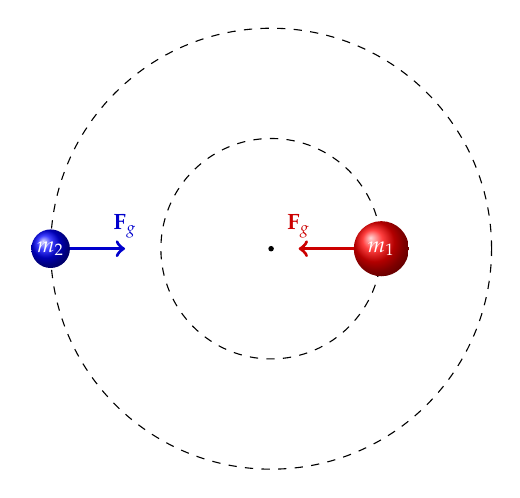
\begin{tikzpicture}[scale=.35]
      \fill(0,0) circle(.1);
      \draw[dashed](0,0) circle(4);
      \draw[dashed](0,0) circle(8);
      \tikzstyle{balloon1}=[ball color=red];
      \tikzstyle{balloon2}=[ball color=blue];
      \shade[balloon1] ( 4,0) circle(1)  node[white]{\footnotesize $m_1$};
      \shade[balloon2] (-8,0) circle(.7) node[white]{\footnotesize $m_2$};
      \draw[very thick,->,blue!80!black](-7.3,0)--(-5.3,0)
      node[pos=1,above]{\footnotesize $\mb{F}_g$};
      \draw[very thick,->,red!80!black](3,0)--(1,0)
      node[pos=1,above]{\footnotesize $\mb{F}_g$};
    \end{tikzpicture}

    \column{.55\textwidth}
    In a binary star system, two stars orbit around their center of mass. Both
    have the same period, and the gravitational force provides the centripetal
    force, but this time, the distance to the center of motion is empty space.
  \end{columns}
\end{frame}

\end{document}
